\chapter{Hierarchical Task Network Planning}
\label{chapter2}
% Hierarchical reasoning is considered to be essential so as to allow humans to manage the complexity of making decisions during their lives. Hierarchical planning is proposed to capture this ability, its basic idea is to supply a planner with a set of high-level actions (HLA), so that the planners can search in a higher level, which makes the planner more effective.

Hierarchical Task Network (HTN) planning has some similarities to classical planning (explained in \autoref{PlanningTechniques}): each state of the world is represented by a set of predicates, and each action defines a deterministic state transition. However, HTN planning techniques differs from classical planning approaches in what they plan for and how they plan for it.

In this chapter, firstly, we explain the HTN technique; then we give the algorithm of an abstract HTN planning procedure; after that, we introduce a group of best-known HTN planners we studied; finally, we discuss and conclude the contents of this chapter.

\section{Definitions and Principles}
\subsection{Task Network (TN)}
Different from classical planning, HTN provides another approach to represent a plan. A task network is a directed acyclic graph. In this graph, each node is a task, the arcs represent precedence ordering between tasks. 

In \autoref{fig2_1}, the nodes $\emph{A, B, C, \ldots}$ are tasks, some orderings are: $\emph{A}$ $\prec$ $\emph{B}$, $\emph{B}$ $\prec$ $\emph{C}$, $\emph{B}$ $\prec$ $\emph{D}$, $\emph{E}$ $\prec$ $\emph{C}$. A task network can be partially ordered. There exists several possibilities when executing a partially ordered plan. For example, there is no ordering constraints between $\emph{C}$ and $\emph{D}$, their execution order is either $\emph{C}$ $\prec$ $\emph{D}$, or $\emph{D}$ $\prec$ $\emph{C}$.%, or $\emph{C}$ and $\emph{D}$ in parallel.

\begin{figure}[H]
    \center
    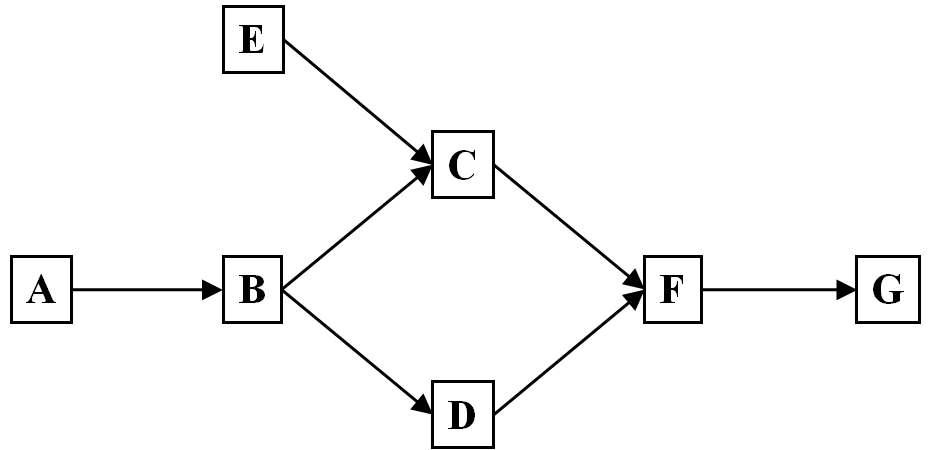
\includegraphics[width=0.6\textwidth]{./images/2_1.png}
    \caption{HTN Example}
    \label{fig2_1}
\end{figure}

\subsection{Hierarchical Structure}
HTN has a hierarchical structure with two kinds of tasks: $\emph{primitive task}$ and $\emph{compound task}$. In \autoref{fig2_1}, each node (e.g. A, B, C, $\ldots$) is either a primitive task or a compound task. 

A \textbf{Primitive Task} is a task that can be achieved directly by executing a corresponding action.

A \textbf{Compound task} is a high-level action (HLA) which must be refined to a group of primitive tasks before execution.

\label{compound_task_example}
In \autoref{fig2_1_1}, the compound task is to reverse a stack, this compound task needs several primitive tasks to be achieved.

\begin{figure}[H]
    \center
    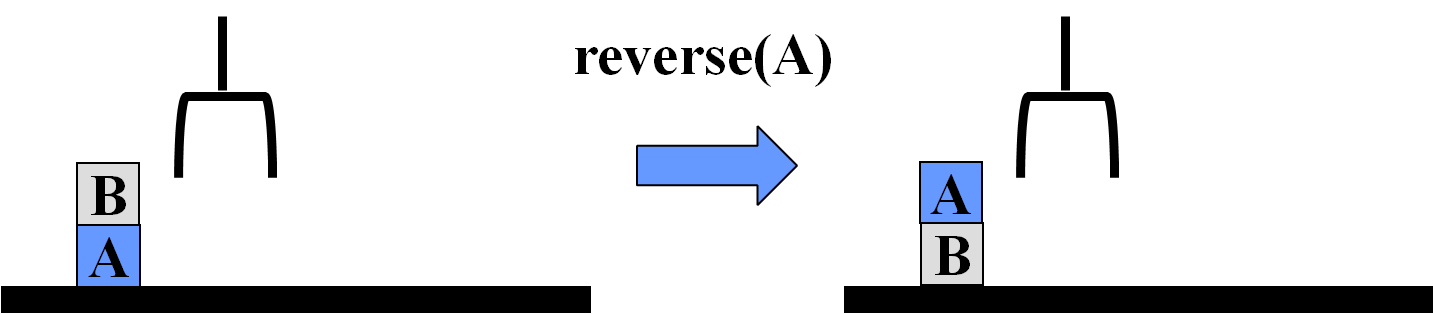
\includegraphics[width=0.8\textwidth]{./images/2_1_1.png}
    \caption{Compound Task Example}
    \label{fig2_1_1}
\end{figure}

% In \autoref{fig2_1_2}, the compound tasks insert(x, y) is to insert a block x into a stack, block y is in the stack, x will be placed on top of y.

% \begin{figure}[H]
%     \center
%     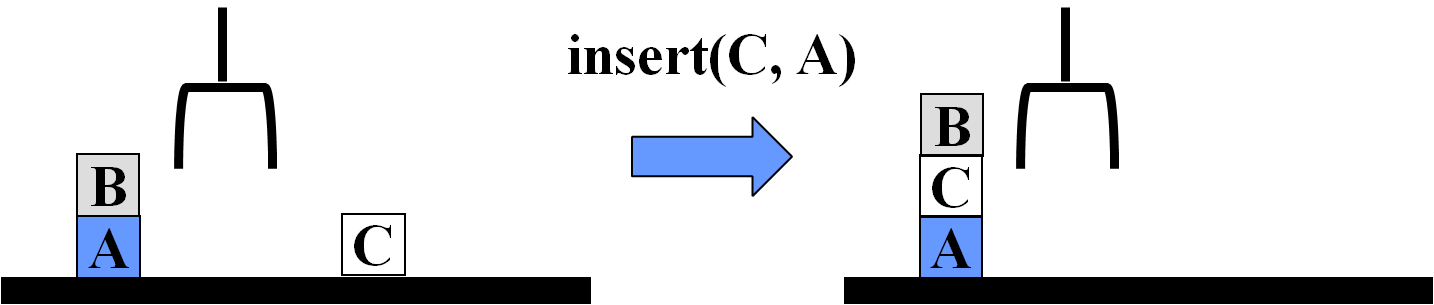
\includegraphics[width=0.8\textwidth]{./images/2_1_2.png}
%     \caption{Compound Task Example 2}
%     \label{fig2_1_2}
% \end{figure}

In \autoref{fig2_1_3}, the compound tasks Clear(x) is to achieve the predicate {\em clear(x)}, it has several possible refinements which lead to different states.

\begin{figure}[H]
    \center
    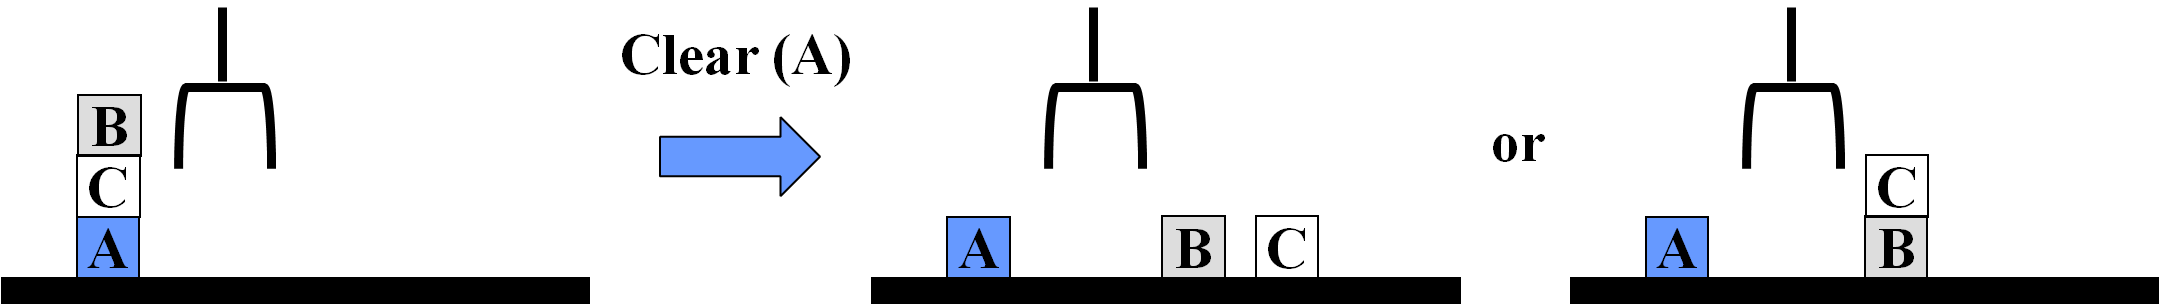
\includegraphics[width=\textwidth]{./images/2_1_3.png}
    \caption{Compound Task Example 2}
    \label{fig2_1_3}
\end{figure}

\subsection{Constraints}
\label{sec:constraints}
In HTN planning, constraints are used to constrain the HTNs. There are two kinds of constraints$\cite{3}$, if n and n' are tasks’ labels in a HTN,
\begin{itemize}
\item[$\bullet$] \textbf{Ordering Constraint}. Ordering constraints are of the form \textbf{n $\prec$ n'}, it indicates that n must finish before n' starts. n and n' both can be primitive task or compound task.

In a more general case, instead of an individual node label like n or n', we use \textbf{first}[$n_i, n_j, \ldots$] and \textbf{last}[$n_i, n_j, \ldots$] to refer to the first task and the last one in execution respectively.

\item[$\bullet$] \textbf{State Constraint}.p is a predicate,
state constraints are as follows:
    \begin{itemize}\itemsep0pt \parskip0pt \parsep0pt
    \item[-] \textbf{Before constraint} is of the form \textbf{(n, p)}, which indicates that predicate p must be satisfied before the task n starts;
    \item[-] \textbf{After constraint} is of the form \textbf{(p, n)}, it indicates that p must be satisfied after the task n finishes.
    \item[-] \textbf{Between constraint} is of the form \textbf{(n, p, n')}. It indicates that p must be true in all states between n and n'.
    \end{itemize}
\end{itemize}

A \textbf{causal link} reflects the interaction between two tasks. $a_i$ and  $a_j$ are tasks in a HTN, a causal link is noted as : $a_i \stackrel{p}{\longrightarrow} a_j$, p is a predicate which is part of  $a_j$’s precondition, the causal link indicates that p is satisfied by executing $a_i$ (i.e. p is part of $a_i$’s effect) and the order $a_i \prec a_j$.

There is a $flaw$ if a state constraint is not satisfied. There are two kinds of flaws, threat and open-link. A threat breaks a causal link.
\begin{itemize}\itemsep0pt \parskip0pt \parsep0pt
\item[$\bullet$] A \textbf{threat} is noted as : $a_k, a_i \stackrel{p}{\longrightarrow} a_j$, $a_k$ is an action which threatens the causal link $a_i \stackrel{p}{\longrightarrow} a_j$, i.e. $\neg$p is part of  $a_k$’s effect, and $a_k$ is ordered between $a_i$ and $a_j$.
\item[$\bullet$] An \textbf{open link} is noted $a_s : \stackrel{p}{\longrightarrow} a_i$, $a_i$’s precondition is not satisfied, p is the corresponding predicate.
\end{itemize}

\subsection{Hierarchical Task Network (HTN)}
A HTN is a collection of $tasks$ together with $constraints$, which is represented as: ( ($n_1$: $t_1$) \ldots ($n_m$: $t_m$), $\emph{C}$ ), where\\
- each $t_i$ is a task;\\
- $\emph{C}$ is a set of constraints;\\
- each $n_i$ is a label for the task $t_i$.

\begin{figure}[H]
    \center
    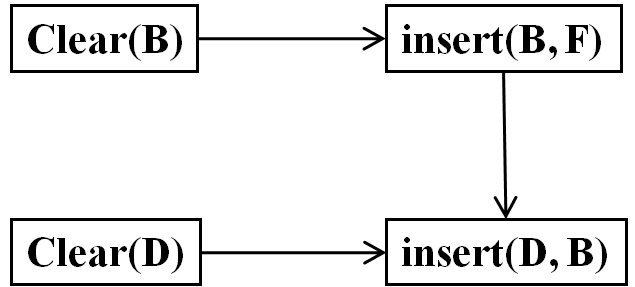
\includegraphics[width=0.4\textwidth]{./images/4_2.png}
    \caption{An example HTN: $t_1$}
    \label{fig4_2}
\end{figure}

The HTN $t_1$ in \autoref{fig4_2} is represented as:\\[0.2cm]
( ($n_1$: Clear(B)) ($n_2$: insert(B, F)) ($n_3$: Clear(D)) ($n_4$: insert(D, B)),  ($n_1$ $\prec$ $n_2$) $\wedge$ ($n_3$ $\prec$ $n_4$) $\wedge$ ($n_2$ $\prec$ $n_4$) $\wedge$ ($n_1$, clear(B)) $\wedge$ ($n_3$, clear(D)) $\wedge$ ($n_2$, on(B,F)) $\wedge$ ($n_4$, on(D,B)) )

% The task $\emph{Clear(B)}$ has many possible refinements, one of them is ( ($n_1$: reverse(B)), ($n_1$, clear(B)) ).

% An example of $t_1$’s effect is in \autoref{fig4_3}:

% \begin{figure}[H]
%     \center
%     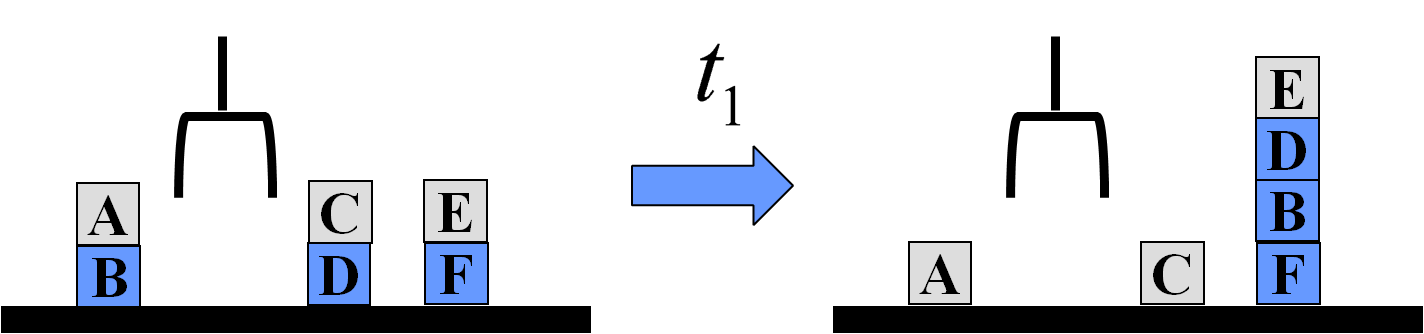
\includegraphics[width=0.8\textwidth]{./images/4_3.png}
%     \caption{An effect example of $\emph{t}$}
%     \label{fig4_3}
% \end{figure}

\subsection{Method}
Each method specifies a way to decompose a compound task into a set of subtasks through associating the compound task with a HTN (i.e. its refinement). A compound task can have several relevant methods (i.e. has several possible refinements). A refinement of a compound task can still contain compound tasks, a method can even be recursive.

% For example, x,y are blocks, a method contains:
% \begin{itemize}
% \item[] \textbf{associated compound task} : reverse(x)
% \item[] \textbf{precondition} : on(y,x)
% \item[] \textbf{refinement} : reverse(y) $\prec$ pickup(x) $\prec$ stack(x,y)
% \end{itemize}

We have extended PDDL to support HTN, an example method defined in PDDL is as the follows:\\[0.2cm]
\hspace*{1cm}(:method reverse\\
\hspace*{1.5cm}  :parameters  (?x - block)\\
\hspace*{1.5cm}  :precondition(and (handempty) (on ?y ?x) (ontable ?x))\\
\hspace*{1.5cm}  :expansion  (\\
\hspace*{2cm}        (tag a (reverse(?y)))\\
\hspace*{2cm}        (tag b (pickup(?x)))\\
\hspace*{2cm}        (tag c (stack(?x, ?y)))\\
\hspace*{1.5cm}  )\\
\hspace*{1.5cm}  :constraints(\\
\hspace*{2cm}        (series a b c)\\
\hspace*{2cm}        (after (and (handempty) (ontable ?x) (clear ?x) (clear ?y)) a)\\
\hspace*{1.5cm}  )\\
\hspace*{1cm})

The name of a method is the same to its corresponding compound task. In the example, the method contains:
\begin{itemize}\itemsep0pt \parskip0pt \parsep0pt
\item[] \textbf{relevant compound task} : $reverse(?x$ - $block$)
\item[] \textbf{precondition} : handempty $\wedge$ on(y, x) $\wedge$ (ontable(x)
\item[] \textbf{refinement} : ( (a: reverse(y)) (b: pickup(x)) (c: stack(x, y)),  (a $\prec$ b) $\wedge$ (b $\prec$ c) $\wedge$ (a, handempty) $\wedge$ (a, ontable(x)) $\wedge$ (a, clear(x)) $\wedge$ (a, clear(y)) )
\end{itemize}

A refinement consists of an $expansion$ (i.e. the set of subtasks) and a group of constraints. In an expansion, “tag” is the key word to indicate the label of a task. A label is necessary, since the same task instance may repeat in a HTN, the labels help to identify the tasks in the constraints, a label can not repeat within a method. In the constraints, “series” is a key word to indicate the ordering constraints, in the example, the ordering of tasks is reverse(y) $\prec$ pickup(x) $\prec$ stack(x, y). “after” is to indicate an after state constraint. When task stack(x, y) finishes, (handempty) $\wedge$ (ontable x) $\wedge$ (clear x) must be satisfied. Other key words “before” and “between” indicate the corresponding constraints. Other method definitions are in \autoref{htnDomain}.

Methods provide additional knowledge to the planning process. A HTN planner do not need to search a complete state-space but to try several known possible decompositions. Thus, HTN’s search space has been reduced compared with classical planning.

\subsection{HTN Planning}
% \autoref{fig2_2} shows the basic procedure of HTN planning. Backtracks happen when a plan does not lead to an implementation, so other paths will be tried.

% \begin{figure}[H]
%     \center
%     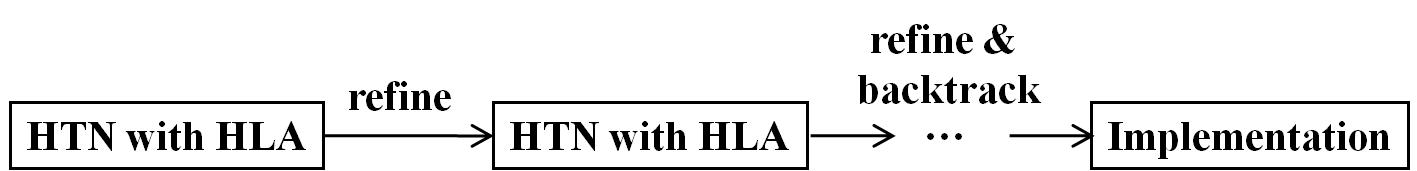
\includegraphics[width=\textwidth]{./images/2_2.png}
%     \caption{HTN Planning Procedure}
%     \label{fig2_2}
% \end{figure}
Some differences between HTN planning and classical planning are as follows:

\begin{table}[h]
    \begin{center}
    \begin{tabular}{|p{1.7cm}|p{4.5cm}|p{5cm}|}%{|c||c|c|}
    \hline
    & Classical Planning & HTN Planning \\
    \hline
    Objective & Achieve a goal state & Perform a task \\
    \hline
    Planning procedure & Search for a sequence of actions that lead to the goal state & Incrementally refine the tasks until reaching an implementation \\
    \hline
    \end{tabular}
    \end{center}
    \caption{Classical Planning vs HTN Planning}
\end{table}

Different from state-space planning, HTN planning searches in plan-space, each node in the search space is a partially-specified plan, each arc is a refining procedure. \textbf{Refining} is the procedure of replacing a compound task with its refinement and updating the corresponding constraints. An \textbf{implementation} is a refinement of a HTN which contains only primitive tasks.

An HTN planning domain consists of a set of operators and a set of methods. Planning process proceeds by refining compound tasks into smaller and smaller tasks, until an implementation has been achieved which can be performed directly.

% All the Classical Planning problems can be translated to HTN planning problems, HTN planning is even more expressive compared to Classical Planning. For example, we need to reverse a stack and then reverse it back as in \autoref{fig2_2_1}. Obviously, the initial HTN is “reverse(A) $\prec$ reverse(B)”, then we can get a solution plan. But in classical planning, the problem will be as in \autoref{fig2_3}, we will always get an empty plan since the goal state is right the same as the initial state.

% \begin{figure}[H]
%     \center
%     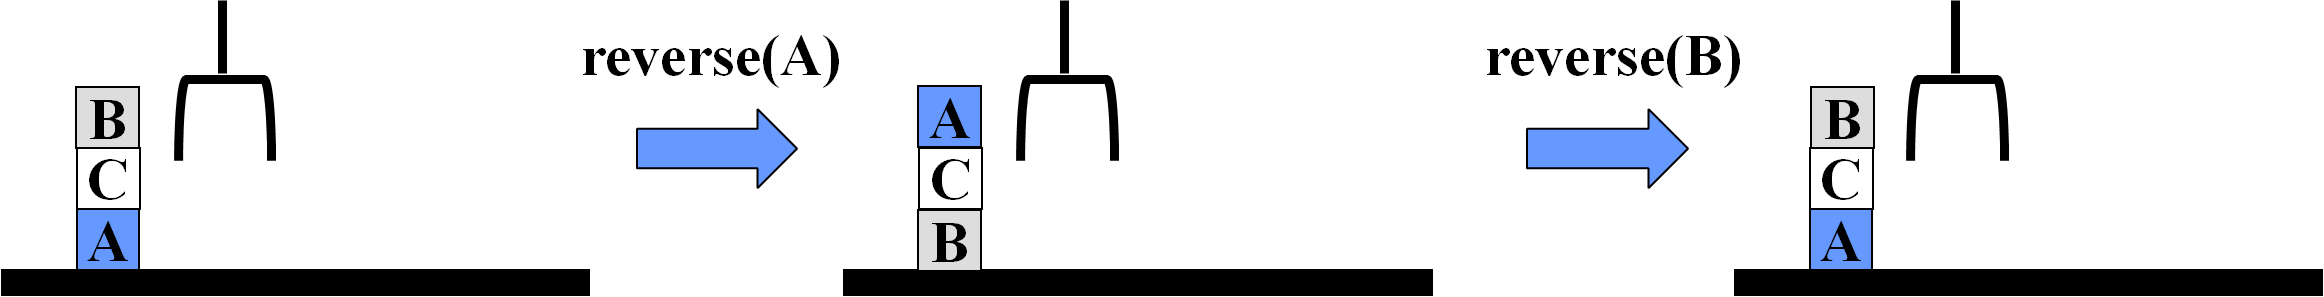
\includegraphics[width=\textwidth]{./images/2_2_1.png}
%     \caption{Expressivity Example: HTN}
%     \label{fig2_2_1}
% \end{figure}

% \begin{figure}[H]
%     \center
%     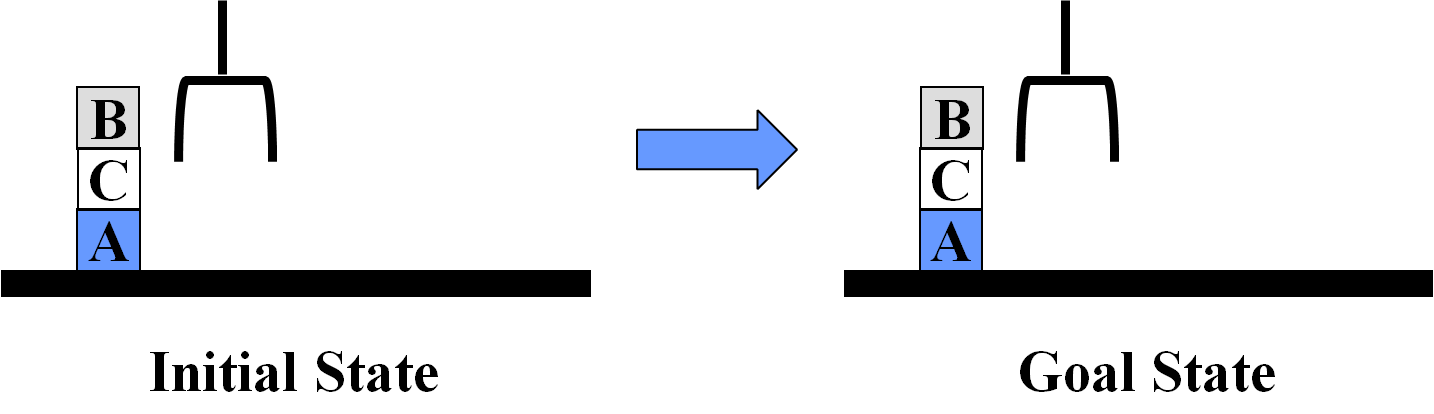
\includegraphics[width=0.8\textwidth]{./images/2_3.png}
%     \caption{Expressivity Example: Classical Planning}
%     \label{fig2_3}
% \end{figure}

% The final state does not change compared to initial state, a classical planner always returns an empty plan.

% The drawback of HTN mainly lies on the difficulties of building a complete domain. All possible refinements of each compound task must be defined in the domain file, if not, there is no way to get good solutions even if with a perfect planner. An example HTN domain is in \autoref{htnDomain}.

\section{Abstract HTN Planning Procedure}
Before introducing the abstract HTN planning procedure, we give some definitions firstly as follows:

% A {\em task} is an expression of the form $t(r_1,\ldots, r_k)$ such that $t$ is a task symbol, and $r_1, \ldots, r_k$ are objects. If $t$ is an operator symbol, then the task is {\em primitive}; otherwise, it is {\em non-primitive}. An action $a = (name(a), precond(a), effect(a))$ {\em accomplishes} a ground primitive task $t$ in a state $s$ if $name(a) = t$ and $a$ is applicable to $s$.

A \textbf{HTN} is a pair $w = (U, C)$, where $U$ is a set of tasks and $C$ is a set of constraints.

A \textbf{method} is a 3-tuple $m = (task(m), expansion(m), constr(m))$ in which the elements are described as follows:
\begin{itemize}\itemsep0pt \parskip0pt \parsep0pt
\item $task(m)$ is the relevant compound task,
\item $expansion(m)$ is a set of subtasks,
\item $constr(m)$ is a a set of constraints,
\item $(expansion(m), constr(m))$ is a HTN to refine to.
\end{itemize}

Suppose that $w = (U,C)$ is a HTN, $u \in U$ is a task, $m$ is a method instance and $task(m) = u$. Then $m$ refine $u$ into $expansion(m)$, producing the HTN
$$
\sigma(w,u,m) = ((U \ - \ \{u\}) \ \cup \ expansion(m), \ C' \ \cup \ constr(m))
$$
where $C'$ is the following modified version of $C$. $p$ is a predicate, $v$ is another task in $w$, the modification is shown as follows, the item before “$\rightarrow$” is the constraint to be replaced, the one after is its replacement.
\label{getC}
\begin{itemize}\itemsep0pt \parskip0pt \parsep0pt
\item[$\bullet$] \textbf{After constraint} ($u$, p) $\rightarrow$ (last[$expansion(m)$], p)
\item[$\bullet$] \textbf{Before constraint} (p, $u$) $\rightarrow$ (p, first[$expansion(m)$])
\item[$\bullet$] \textbf{Between constraint} 
    \begin{itemize}\itemsep0pt \parskip0pt \parsep0pt
    \item[-] ($v, p, u$) $\rightarrow$ ($v$, p, first[$expansion(m)$])
    \item[-] ($u, p, v$) $\rightarrow$ (last[$expansion(m)$], p, $v$)
    \end{itemize}
\item[$\bullet$] \textbf{Ordering constraint}
    \begin{itemize}\itemsep0pt \parskip0pt \parsep0pt
    \item[-] ($v \prec u$) $\rightarrow$ ($v \prec$ first[$expansion(m)$])
    \item[-] ($u \prec v$) $\rightarrow$ (last[$expansion(m)$] $\prec v$)
    \end{itemize}
\end{itemize}

An HTN \textbf{planning problem} is a 4-tuple ${\cal{P}} = (s_0, w, O, M)$ where $s_0$ is the initial state, $w$ is the initial HTN, $O$ is a set of operators, and $M$ is a set of methods.

A \textbf{linearization} of a partially-ordered plan is a totally-ordered plan which satisfies all the ordering constraints of the partially-ordered plan. For example, the plan (or HTN) in \autoref{fig4_1} has two linearizations: $\emph{A}$ $\prec$ $\emph{B}$ $\prec$ $\emph{C}$ and $\emph{A}$ $\prec$ $\emph{C}$ $\prec$ $\emph{B}$.

\begin{figure}[H]
    \center
    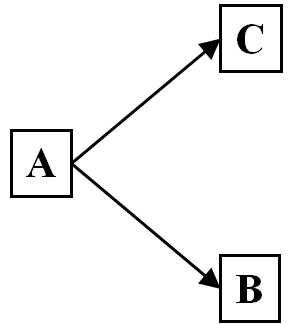
\includegraphics[width=0.19\textwidth]{./images/4_1.png}
    \caption{A partially-ordered plan}
    \label{fig4_1}
\end{figure}

A \textbf{solution plan} is a partially-ordered plan, each of its linearizations satisfies all the state constraints of the HTN.

An abstract HTN planning procedure is as follows:

\begin{algorithm}[H] 
\caption{Abstract HTN Planning Procedure}
\label{Algo:HTN}

\SetKwFunction{HeuristicForwardSearch}{Heuristic-forward-Search}
\SetKwData{Failure}{failure}
\SetKwData{Active}{active}
\SetKwData{Open}{open}
\SetKwData{Continue}{continue}
\KwIn{a planning problem ${\cal{P}} = (s_0, w, O, M)$} 

\Open $\leftarrow$ \{$w$\} \;

\While{\Open $\ne \emptyset$} {
  nondeterministically choose a HTN $\nu \in \Open$ \;
  remove $\nu$ from \Open\;
  \eIf{$\nu = (U, C)$ is primitive}{
    \lIf{all constraints in $C$ are satisfied}{\Return $\nu$}
    % \lElse{\Continue}
  }{
    nondeterministically choose a task $u \in \nu$ \;
    \Active $\leftarrow \{ m \in M \ | \ task(m)$ is relevant to $u \}$ \;
    \If{$\Active \neq \emptyset$}{
      \For{each method $m \in \Active$}{
        $\mu \leftarrow ((U \ $-$ \ \{u\}) \ \cup \ expansion(m), \ C' \ \cup \ constr(m))$\;
        add $\mu$ to \Open\;
      }
    }
    % {
    %   \Return \Failure \;
    % }
  }
}
\Return \Failure \;
\end{algorithm}

In line 1, the algorithm begins with the input initial HTN, which is stored in $open$. $open$ is a list of HTN, it is used to store all the generated HTNs during the search.

In line 3-4, a HTN $\nu$ is popped from $open$, it has been chosen non-deterministically, a deterministic choice will be discussed in \autoref{chapter_heuristic}.

In line 5-6, if the selected HTN is primitive (i.e. an implementation), we check if all the constraints within the HTN has been satisfied, if so, we return the HTN which is a solution.

In line 7-9, if the selected HTN is not an implementation, which means there exists still compound tasks within the HTN. Then one of the compound tasks is chosen non-deterministically, and all its relevant methods will be stored in $active$. A deterministic choice of compound task will also be discussed in \autoref{chapter_heuristic}.

In line 10-13, if $active$ is not empty, each relevant method will be applied, we use $m$ to refine the selected compound task, an updated HTN will be obtained and stored in $\mu$, then it is added in $open$ to be considered in following iterations.

In line 14, if $open$ is empty, which means all possible refinements have been tried without finding a solution, there is no solution to the input planning problem, the algorithm returns failure.

\autoref{Algo:HTN} is sound and complete.

\section{Related Work}
The basic ideas of HTN planning were developed more than 25 years ago in works of Sacerdoti \cite[p. 460]{1} and in Tate's Nonlin planner \cite[p. 503]{1}. HTN planning has been more widely used in planning applications than any other classical planning techniques, e.g., in production line scheduling \cite[p. 549]{1}, crisis management and logistics \cite[p. 72]{1} \cite[p. 135]{1}, etc.

The first step toward a theoretical model of HTN planning is taken by Yang \cite[p. 558]{1} and Kambhampati \cite[p. 301]{1}. A complete model was developed by Erol \cite[p. 174]{1}. This model provided the basis for complexity analysis \cite[p. 175]{1} and the first provably correct HTN planning procedure (the planning procedure \ref{Algo:HTN} is based on this work). 

Some best-known domain-independent HTN planning systems are listed below.
\paragraph*{UMCP}
\label{sec:UMCP}
\cite{3} \cite{3_1} \cite[p. 174]{1} is an implementation of the first provably sound and complete HTN planning algorithm. UMCP searches by iteratively refining a non primitive HTN to a primitive one. In each iteration, a non-primitive task is selected non-deterministically, one of its relevant methods will be chosen to refine it, then according to this refinement, a new HTN is created. Once a primitive HTN is created, it will be returned if all the constraints of the problem are satisfied, or the planner backtracks. To reduce the amount of backtracking, UMCP calls a function for detecting and resolving the flaws caused by interactions among tasks.
% \cite{3} \cite{3_1} (Universal Method-Composition Planner) is the first provably sound and complete HTN planning system. 

% UMCP’s planning domain and problem’s definitions are as follows:

% \textbf{planning domain $\mathcal{D}$}: A planning domain of UMCP is a pair <Op, Me>, Op is the set of operators (each operator instance is a primitive task), and Me is the set of methods.

% \textbf{planning problem} : A planning problem of UMCP is a triple <d, I, $\mathcal{D}$>, $\emph{d}$ is the HTN we need to plan for, $\emph{I}$ is the initial state, and $\mathcal{D}$ is the planning domain.

% In UMCP’s search process, $\emph{d}$ is refined iteratively up to a primitive TN. In each iteration, a compound task of $\emph{d}$ is selected non-deterministically, one of its relevant methods will be chosen to refine the compound task, then according to this refinement, $\emph{d}$ is updated. Once $\emph{d}$ is primitive, it will be returned if all the constraints of the problem are satisfied, or the planner backtracks. To reduce the amount of backtracking, UMCP calls the $\emph{critics}$\cite{3_2}, which is a function for detecting and resolving the flaws caused by interactions among tasks. For example, in \autoref{fig2_3_2}, there are two primitive tasks $\emph{pickup(C)}$ $\prec$ $\emph{putdown(C)}$ and a compound task $\emph{Clear(A)}$, $\emph{Clear(A)}$ aims at achieving the predicate $\emph{clear(A)}$, it has two possible refinments: $\emph{pickup(B)}$ $\prec$ $\emph{putdown(B)}$ and $\emph{pickup(B)}$ $\prec$ $\emph{stack(B,C)}$. There is no ordering constraint between $\emph{pickup(C)}$ and $\emph{Clear(A)}$. If during the planning, $\emph{Clear(A)}$ is refined as $\emph{pickup(B)}$ $\prec$ $\emph{stack(B,C)}$, there is a flaw that the precondition $\emph{clear(C)}$ is violated, $\emph{critics}$ must find this flaw and try to repair it. One way to repair a flaw is to add ordering constraints, as in \autoref{fig2_3_2}, we may add ordering constraint $\emph{putdown(C)}$ $\prec$ $\emph{stack(B,C)}$. Another way to repair a flaw is to try another refinement of the current compound task. As in \autoref{fig2_3_2}, $\emph{critics}$ may force the planner to refine $\emph{Clear(A)}$ as $\emph{pickup(B)}$ $\prec$ $\emph{putdown(B)}$, then the flaw is resolved. If $\emph{critics}$ can not repair a flaw, it forces a backtrack, since further refining is senseless. 

% \begin{figure}[H]
%     \center
%     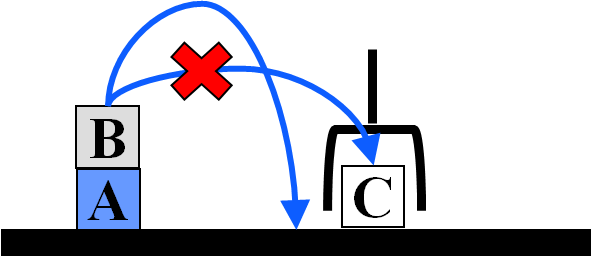
\includegraphics[width=0.4\textwidth]{./images/2_3_2.png}
%     \caption{A HTN with a ordering circle}
%     \label{fig2_3_2}
% \end{figure}

% UMCP checks with $\emph{critics}$ frequently, it is performed in each iteration of the search process, so as to detect interactions early and to end meaningless search as soon as possible (i.e. to end the refining on a plan which will never lead to a solution), so that both the amount of backtracking and the size of search space are reduced.

\paragraph*{SHOP}
\label{sec:SHOP}
\cite{4} \cite{4_1} (Simple Hierarchical Ordered Planner) plans for tasks in the same order as their execution, thus it can always keep track of world-state during the planning process. With the knowledge of the current state, SHOP gains planning efficiency, it refines non-primitive tasks only with the available methods (i.e. a method whose precondition and also the precondition of the first task of the method’s refinement are satisfied), so that the search space is reduced compared to UMCP; it also gains expressive power, since the knowledge of current world-state allows using $\emph{dynamic expressions}$ (e.g. numeric expressions, calling external programs). But these features force SHOP to do a forward search from the first task to the last one as the tasks’ execution ordering, and the result plan is limited to be totally ordered. SHOP is sound and complete, but it suffers from backtracking. When there is no applicable method to decompose a non-primitive task, it backtracks to guarantee the completeness. There can be several possible ways to decompose a non-primitive task, backtracking happens after a non-primitive task has not been decomposed with the proper method. However, in SHOP, methods are chosen non-deterministically, and it is hard to decide which node in the search space to backtrack to. 
\label{sec:SHOP}

\paragraph*{M-SHOP}
\cite{5} (Multi-task-list SHOP) generalizes SHOP by allowing the initial HTN to be partially ordered, thus the refinements of non-primitive tasks may be interleaved when executing the plan. The interleaving allows removing duplicated actions. M-SHOP does not guarantee to remove all the duplicated actions, and the solution plan is not guaranteed to be optimal (i.e. result plan with the smallest length). The interleaving may cause task-interaction issues. To deal with the issue, in M-SHOP, $\emph{protection request}$ and $\emph{protection cancellation}$ are defined in action effects. A protection request is to guarantee a predicate. The predicate guaranteed must be satisfied before the protection is canceled. M-SHOP uses a global list to store the protection list. 

\paragraph*{GoDel}
\cite{godel} (Goal Decomposition with Landmarks) is motivated by the fact that planners have methods which only solve some subproblems, but not the top-level problems. Instead of a HTN, GoDeL uses a goal network as input. A {\em goal network} is a partial order network which guides the algorithm to achieve the final goal step by step, each node in the network is a world state, the final node is the final goal state. The definition of method in GoDeL is also different, it does not have the HTN to refine to, instead, it has a sub goal network to indicate the steps to achieve the goal. In GoDeL, both methods and $\emph{subgoal inference}$ are used to decompose a task to sub-tasks (i.e. add subgoals into the goal network). Subgoal inference is based on landmarks. A {\em landmark} for a planning problem P is a fact that is true at some point in every plan that solves P, so it is considered as a subgoal that every solution to P must satisfy at some point. The algorithm performs a forward search from the initial state, it keeps track of the current state. By combining classical planning and HTN planning, GoDeL supports incomplete domains, no matter the domain knowledge is complete, it is always sound and complete. 


\paragraph*{Angelic}
The basic idea of Angelic \cite{angelic1} is to plan in a higher level. Angelic needs an additional goal description $G$ (a set of literals) to resolve a planning problem and two sets of reachable states called Overstated (i.e. superset) and Understated (i.e. subset). These two sets can be considered as $\emph{MAY}$ and $\emph{MUST}$ reachable states respectively. If $\emph{MUST}$ $\subseteq$ G, ADD A VERB then arbitrary implementation of the HTN achieves the goal. If $\emph{MAY}$ $\cap$ $G = \emptyset$, there is no need to continue to refine the plan which will never lead to the goal state. With deeper refining, a non-primitive task’s reachable states will be exacter, so when goal state is in $\emph{MAY}$ but not in $\emph{MUST}$, the non-primitive tasks in the plan need to be refined. 

The algorithm does a top-down, forward search (i.e. from the top-level non-primitive task to a primitive plan, from the first task to the last one as the tasks’ execution order), it is sound and complete, and the plan is totally-ordered. With the help of non-primitive task description, refining is performed only when it is necessary, so that the algorithm can avoid backtracking.

The extended version$\cite{angelic2}$ of Angelic considers cost of actions, it generates provably optimal plans or generate nearly optimal plans with better performance. Its heuristics is inspired from A* algorithm, the heuristics use the data structure of $\emph{abstract lookahead tree}$ (i.e. lookahead tree adapted for non-primitive task). The algorithm’s basic idea is the same to the original version, each node of the abstract lookahead tree has an $\emph{optimistic cost}$ and a $\emph{pessimistic cost}$, the optimistic cost will be infinite for the nodes from which the goal states is unreachable. So the plan with the lowest optimistic cost will be refined prior to others. When an exact cost is obtained, the plans whose optimistic cost is greater than the obtained value will no longer be considered.

\paragraph*{Yoyo}
The main idea of Yoyo\cite{yoyo} is to combine HTN with BDD (Binary Decision Diagram) for planning in non-deterministic domain. In non-deterministic domain, each action can have several alternative effects (i.e. the actual effect of an action is randomized), but the plan must work despite the non-determinism, so all possible effects (or all possible following states) must be considered, any state which leads to a $\emph{dead end}$ (i.e. no further refining can be done, but the goal state is not yet achieved) forces the algorithm to return a failure. 

To guarantee that every execution path (multiple execution path is caused by different action effect) leads to the goal state, the returned plan is also different from other planners, it returns a list of situations (a situation is a pair of state and action), it indicates appropriate action according to the observed state. Yoyo does a forward search, in each iteration of the algorithm, it chooses a task without predecessor in the HTN, and it searches with the knowledge of the current state, so only applicable actions are considered in each step. Yoyo is both sound and complete. 

BDD is used to represent a set of states in Yoyo. With the help of BDD, Yoyo realizes a set-based search, so that it avoids to search for each state separately and gains efficiency. To represent a set of states, the BDD does not need to list the propositions for which both arcs lead to the same terminal node, so an appropriate use of BDD also reduces the memory consumption.

\paragraph*{HiPOP}
\cite{hipop} (Hierarchical Partial-Order Planner) combines HTN and partial order planning (POP) [Add ref 50 Ghallab's book]. It supports optional user-defined non-primitive tasks and methods. HiPOP is both sound and complete. 

If there is no non-primitive task defined, HiPOP works in the same way as a classical POP algorithm. The initial plan of classical POP consists of two dummy actions $a_s$ and $a_e$, $a_s$ is the first action of the result plan, and $a_e$ is the last one. Precondition($a_s$) $=$ $\emptyset$, Effect($a_s$) $=$ I; Precondition($a_e$) $=$ G, Effect($a_e$) $=$ $\emptyset$. Obviously, if $I \not\in G$, the plan is initialized with an open-link to repair. All generated plans for repairing a flaw are inserted into an open plan list. For each iteration, a plan which is not yet explored in the open list will be chosen and removed from the open list. According to the heuristics, the chosen plan should be the one which is most likely to be a solution. If the chosen plan does not contain any flaw, it will be returned. Otherwise, one of its flaws will be chosen and repaired. The algorithm stops and returns failure if the open list has been empty while no solution is found.

Extended from classical POP, HiPOP plans with non-primitive task. Each non-primitive task is considered as an $\emph{abstract flaw}$, so a solution plan must be primitive. To take the advantage of non-primitive task, only non-primitive task is allowed to be directly added into the plan for repairing flaws, primitive actions can only be added through refining. In this way, through the additional knowledge provided by methods, the planning is guided as much as possible.

A* algorithm has been used as the plan heuristics. For flaw heuristics, the general order is: threat > open-link > abstract flaw (a > b means that a is prior to b), threats with the fewest resolvers will be solved firstly. Generally, open-links is solved earlier than abstract flaws, so that the algorithm deals with smaller plans during search process. Otherwise, after all the refining have been done, a huge plan with many flaws is likely to be generated.

\paragraph*{IMPACTing SHOP}
\cite{ishop} integrates SHOP and IMPACT \cite{Impact} multiagent environment. In this work, although the environment is a Multiagent System, the planning is centralized, and it supports only a single planner while other agents are considered as information sources. Among IMPACT agents, there exists some special agents such as: statistics agent, monitoring agent, supplier agent which is for supporting calling external functions; math agent which supports numerical expressions.

To support the planner to interact with external agents (i.e. information sources), in the planning algorithm A-SHOP (agentized SHOP), the preconditions and the effects of actions have been replaced with code-calls, a code-call is a function call to other IMPACT agent. Direct execution of these code-calls cause difficulties when the algorithm needs to backtrack, since code-calls affect other agents’ states. To solve this problem, a monitoring agent monitors the code-calls without executing them, the code-calls are actually applied only when the apply function is called.

A code-call is an arbitrary software function, thus the algorithm is sound and complete only when code-calls are $\emph{strongly safe}$, which guarantees the finiteness of a function call.

\paragraph*{CoRe Plannner}
\cite{multi2} has a multiagent planning model which cooperates agents for achieving a common goal. The system has combined the advantages of POP and HTN, POP is adapted to concurrent planning in distributed environment, HTN has advantages in both efficiency and expressivity. Agents’ partial knowledge and heterogeneous skills are also supported in the system.

The system plans for achieving a given goal state G, all the agents search within a global shared search space. The search space is represented with a Directed Acyclic Graph (DAG), whose nodes are partial plans. The nodes are allowed to contain flaws which are considered as promises, the flaws become new goals in the following planning. Each agent can refine, refute or repair a partial plan (i.e. a node in the DAG), and records other agents’ propositions. 

The initial plan is the same as in Classical POP ( in explanation of HiPOP). Then in each iteration of the algorithm, one of the $\emph{non-terminal plans}$ (i.e. at least one refining or repair or refutation is applicable) which is not yet explored will be chosen. If the chosen plan does not contain any flaw, the agent proposes a “success”. Otherwise, one of its flaws will be chosen, if the flaw is an open-link, it will be solved by adding a causal link or by the HTN-based refinement mechanism; if the flaw is a threat, the system will try to repair it. All the generated plans for solving a flaw are added in the DAG.

When an agent proposes a “success” (resp. failure) and wait for responses of other agents, the other agents verify whether the proposed plan is a solution plan (resp. whether this agent is not able to provide a possible solution) with their own knowledge. If the proposition is accepted by all the agents, the planning process ends. Otherwise, the system goes back to the planning phase.

The system is both sound and complete. The solution plan is partially-ordered. A* algorithm is applied as the plan heuristics. For flaw heuristics, a flaw with the fewest resolvers will be chosen. 

\section{Discussion and Conclusion}
Compared with classical planners, the primary advantage of HTN planner is their additional knowledge representation and reasoning capabilities. With a good set of methods, HTN planners can solve classical planning problems orders of magnitude more quickly than classical planners. 

All the Classical Planning problems can be translated to HTN planning problems, HTN planning is even more expressive than classical planning. HTN planners can represent and solve a variety of non-classical planning problems. For example, we need to reverse a stack and then reverse it back as in \autoref{fig2_2_1}. Obviously, the initial HTN is “reverse(A) $\prec$ reverse(B)”, we can get a solution after HTN planning process. However, in classical planning, the problem will be as in \autoref{fig2_3}, we always get an empty plan since the goal state is right the same as the initial state.

\begin{figure}[H]
    \center
    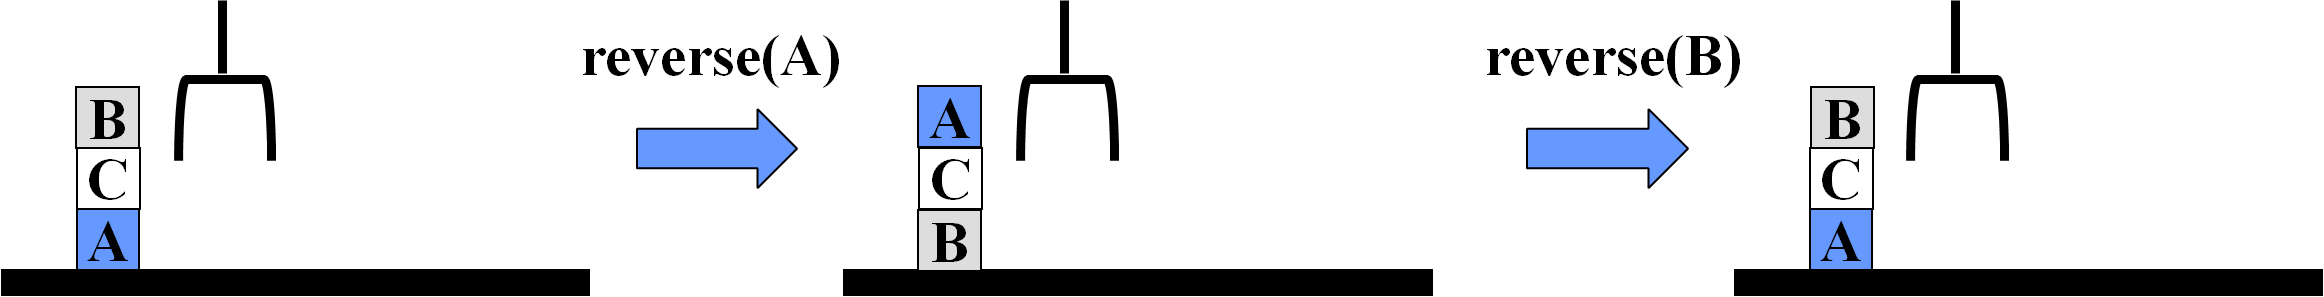
\includegraphics[width=\textwidth]{./images/2_2_1.png}
    \caption{Expressivity Example: HTN}
    \label{fig2_2_1}
\end{figure}

\begin{figure}[H]
    \center
    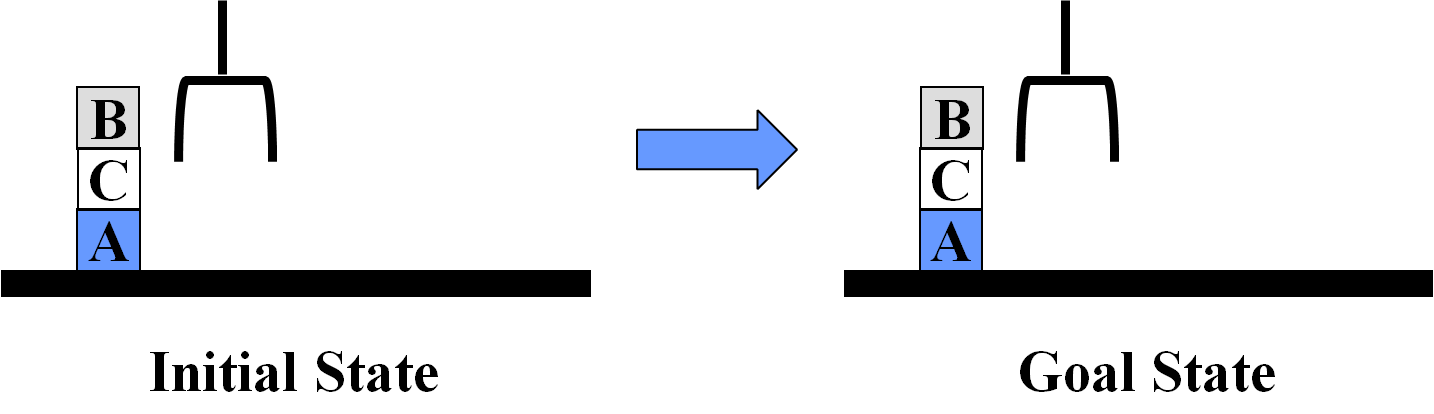
\includegraphics[width=0.7\textwidth]{./images/2_3.png}
    \caption{Expressivity Example: Classical Planning}
    \label{fig2_3}
\end{figure}

The primary disadvantage of HTN planners is the need for the domain author to write not only a set of planning operators but also a set of methods.

The basic ideas of the planners we have studied are as follows: UMCP refines compound tasks in an arbitrary order. SHOP simplifies the planning process to be in the same order as execution. M-SHOP allows un-ordered tasks in initial HTN. GoDeL combines HTN with classical planning to support incomplete domain. Angelic avoids backexpansioning through HLA descriptions. Yoyo combines HTN with BDD to support non-deterministic domains. IMPACTing SHOP combines SHOP with IMPACT to support multiple information sources. Both the CoRe and HiPOP combine POP with HTN.

Among these planners, SHOP, M-SHOP, GoDeL, Angelic, Yoyo and IMPACTing SHOP keep track of the world-state, they do a forward search step by step from the initial state. They loose flexibility, but they gain efficiency, since only available methods will be applied. UMCP chooses arbitrary compound task in a HTN to refine, but it is not as efficient as the planners like SHOP. CoRe and HiPOP both based on POP and HTN, they repair flaws during the planning process, which do not require exact world states, but they are rather POP planners, POP is the base of their planning process, HTN is only a strategy to increase the efficiency. HTN works differently in the two systems, HiPOP uses HTN to support abstract actions, in the CoRe, HTN is used in flaw repairing. The current version of HiPOP only supports single agent planning, while the unified framework is a multiagent planning system.

HTN planning is efficient, expressive, and widely used. However, among the above HTN planners, there is no heuristics except the extended Angelic, whose heuristics is based on HLA description. The heuristics play an important role in automated planning for improving system’s performance, we are proposing our heuristics without the information of HLA description in \autoref{chapter_heuristic}.
